\section{CIFAR-10/100 Benchmarks with Fixed Training Cost}
\label{cifar_sc}
We also compared methods such that each took about the same cost on two virtual machines for 10,000 training samples (Figure \ref{fig:cifar_sc}). The baseline was RF's training times as run on the 2-core Standard\_DS2\_v2 Azure compute instance (Table \ref{table:azure}). The SVM-RBF benchmarks were also run on the same compute instance for reference. As a result, the training wall times of CNNs, which often used the minimum epoch number, were always lower than those of RF. Due to the CNNs' different complexities, the correspondence between training costs became more accurate as the class number increased. The networks' training time trajectories also overlapped more completely. The results were qualitatively similar to CIFAR benchmarks with fixed training time (Figure \ref{fig:cifar_st}).

\begin{figure}[!htb]
\centering
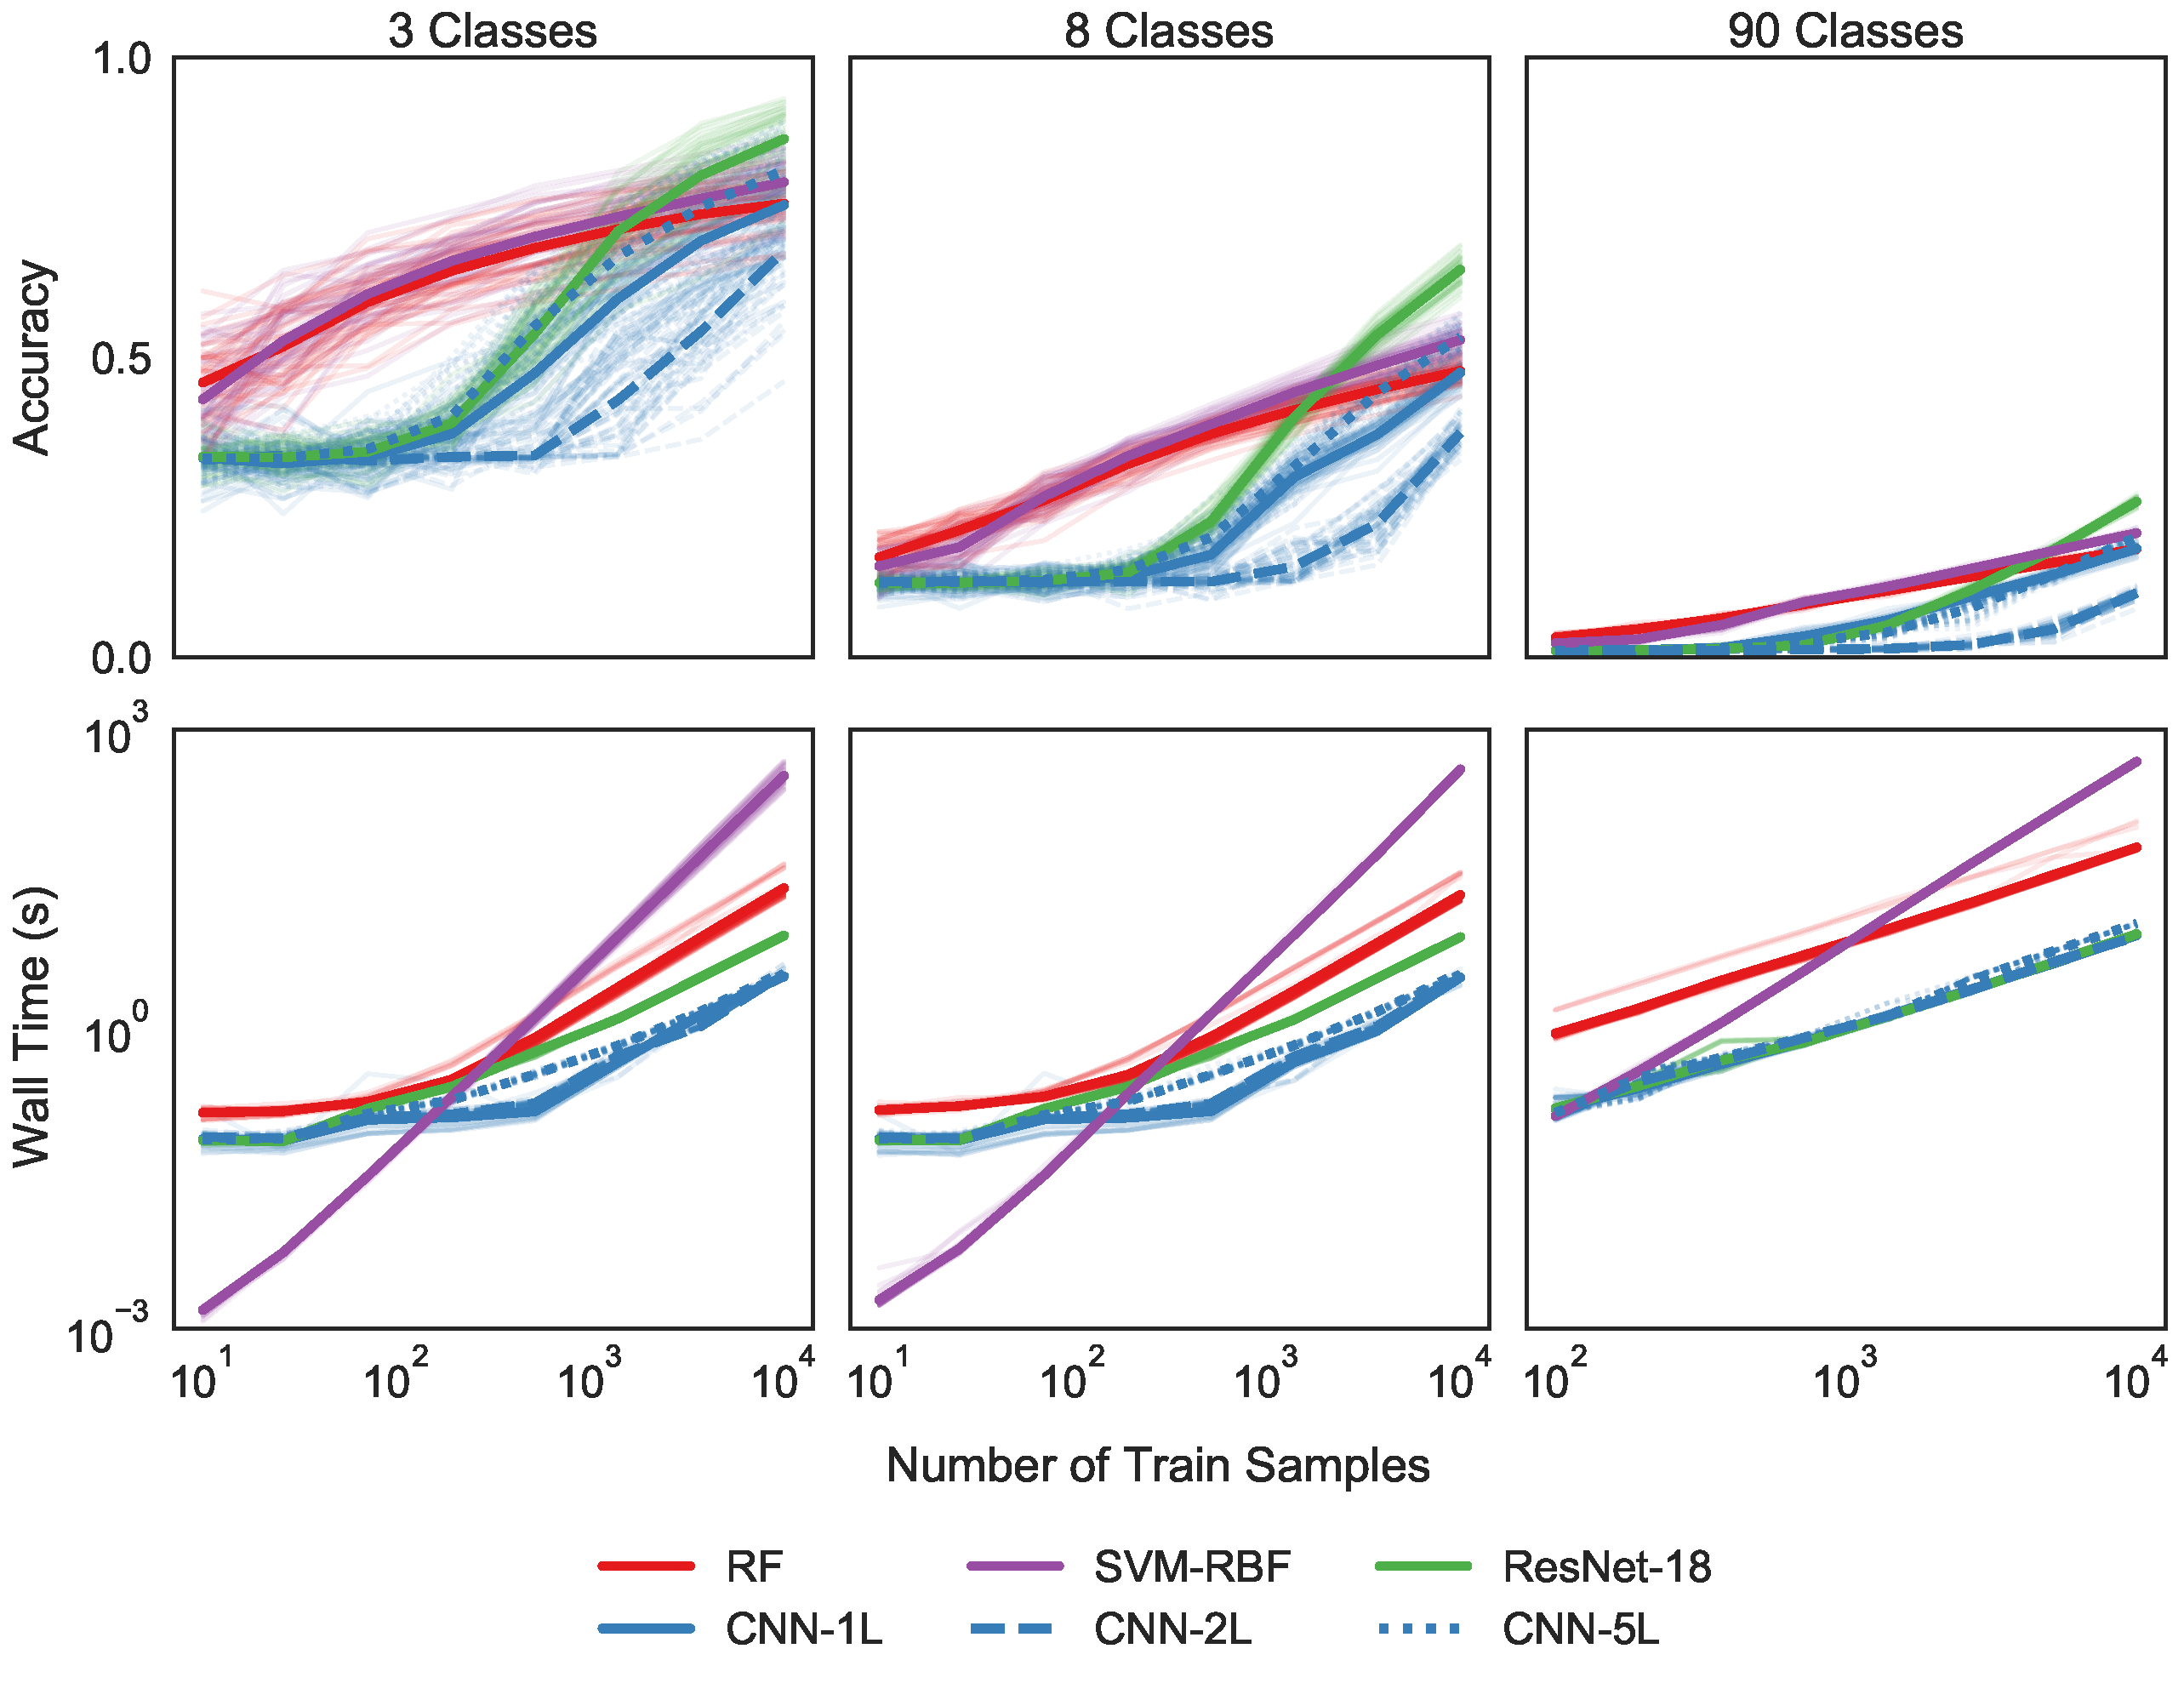
\includegraphics[width=0.8\textwidth]{figures/cifar_sc.pdf}
  \caption{Performance of RF, SVM-RBF, and DN on multiclass CIFAR-10/100 classifications with fixed training cost.
  Upper row represents classifier accuracy on a linear scale, and bottom row represents training wall times in seconds on a logarithmic scale. The x-axes correspond to logarithmic sample sizes for respective columns. Each panel shows average results over 45 random combinations. The left two columns use CIFAR-10, while the rightmost uses CIFAR-100.
  RF and SVM-RBF have higher classification accuracy and lower training wall times compared to CNNs at smaller sample sizes. Complex networks, however, surpass RF and SVM-RBF at larger sample sizes, and ResNet-18 always performs best in the end.
  }
\label{fig:cifar_sc}
\end{figure}
\vfil\eject

\section{SVHN Benchmarks}
\label{svhn}
The SVHN dataset contains 73,257 digits for training and 26,032 for testing \citep{svhn}. The 3-class and 8-class tasks showed surprising trends for DN, as simpler CNNs surpassed ResNet-18 as the sample size increased. At higher sample sizes, the CNN with five convolutional layers had the best performance among all classifiers. DN accuracy was always higher than that of RF and SVM-RBF at the max sample size (Figure \ref{fig:svhn}). Although RF and SVM-RBF could perform better than DN at smaller sample sizes in the 3-class task, the advantage disappeared in the 8-class task. As seen in the CIFAR benchmarks, DN would be more adept at handling higher class numbers.

The trends of training wall times were very similar to those of CIFAR benchmarks with unbounded time and cost (Figure \ref{fig:cifar}). RF's training times were always shorter than DN's, and more fluctuations occurred for CNN trajectories.

\begin{figure}[!htb]
\centering
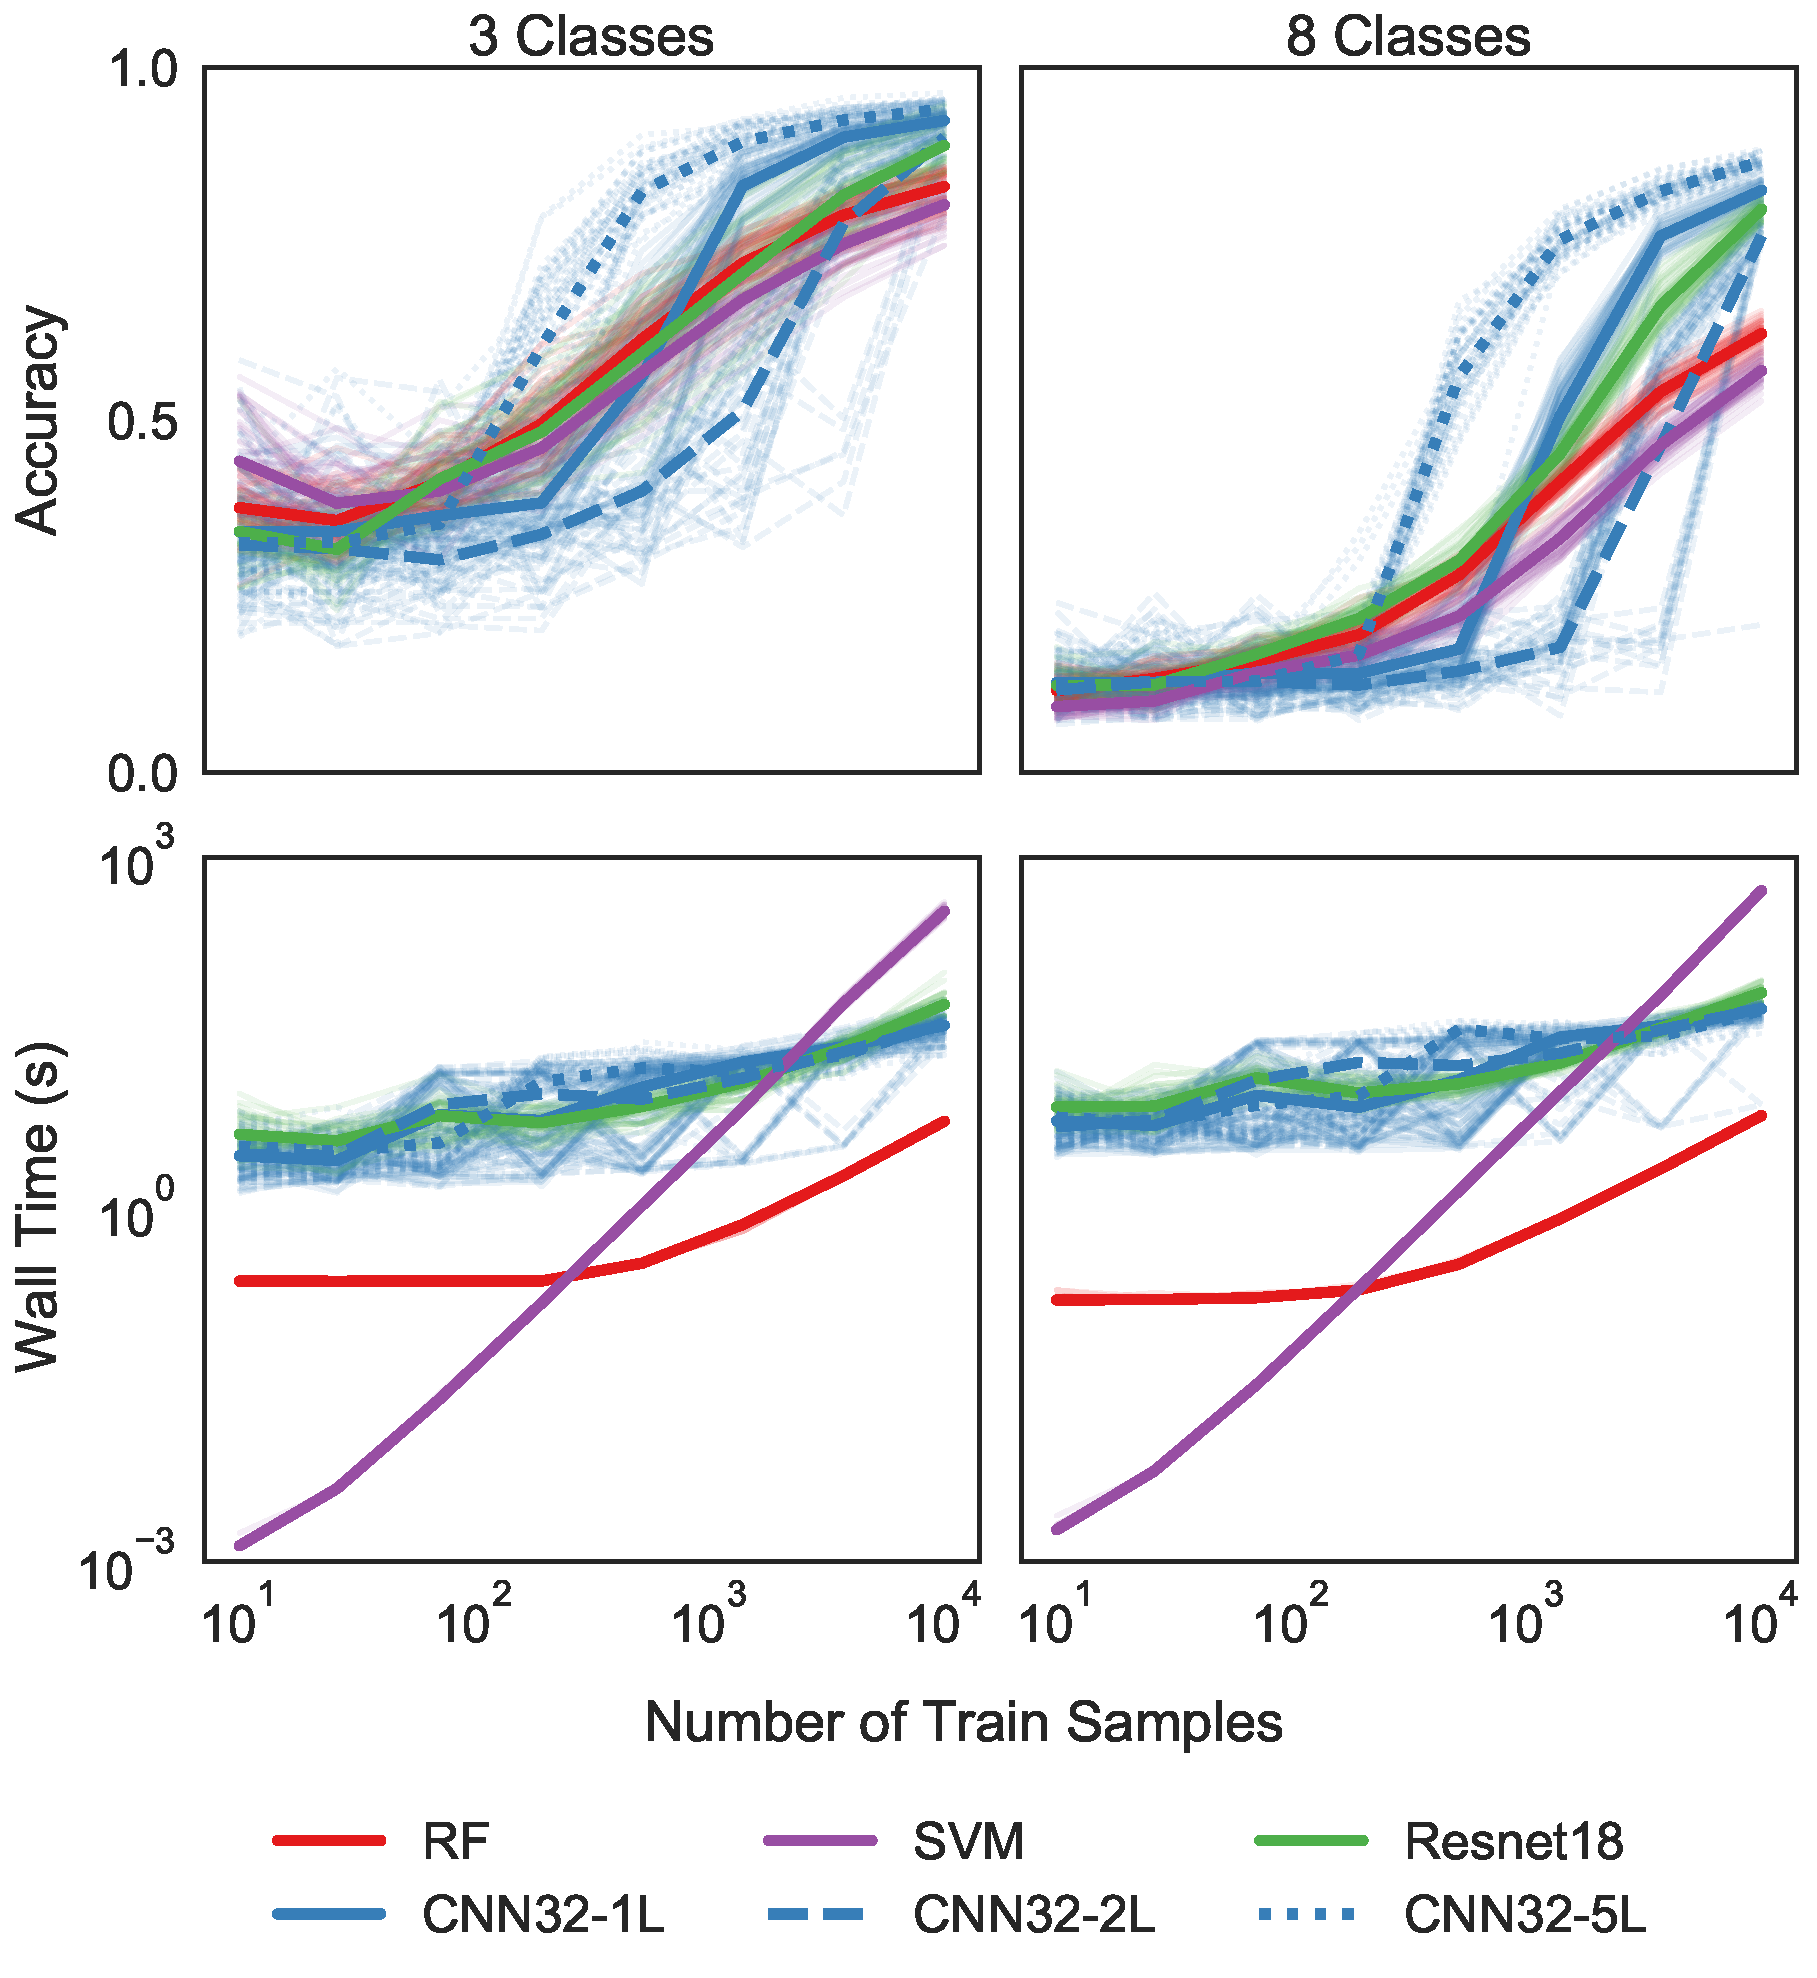
\includegraphics[width=0.6\textwidth]{figures/svhn.pdf}
  \caption{Performance of RF, SVM-RBF, and DNs on multiclass SVHN classifications with unbounded time and cost.
  Upper row represents classifier accuracy on a linear scale, and bottom row represents training wall times in seconds on a logarithmic scale. The x-axes correspond to logarithmic sample sizes for respective columns. Each column shows average results over 45 random combinations.
  Compared to CNNs, RF and SVM-RBF perform better and faster at smaller sample sizes.
  }
\label{fig:svhn}
\end{figure}
\vfil\eject

\section{FSDD Benchmarks with Mel-Spectrogram}
\label{mel}
As an alternative approach, we used PyTorch’s inbuilt function and converted the raw audio magnitudes into mel-spectrograms \citep{pytorch}. The process involved the aforementioned spectrogram conversions and used triangular filterbanks to modify the images. The results (Figure \ref{fig:mel}) were qualitatively similar to FSDD benchmarks with spectrogram (Figure \ref{fig:spoken_digit}) and MFCC (Figure \ref{fig:mfcc}) conversions.

\begin{figure}[!htb]
\centering
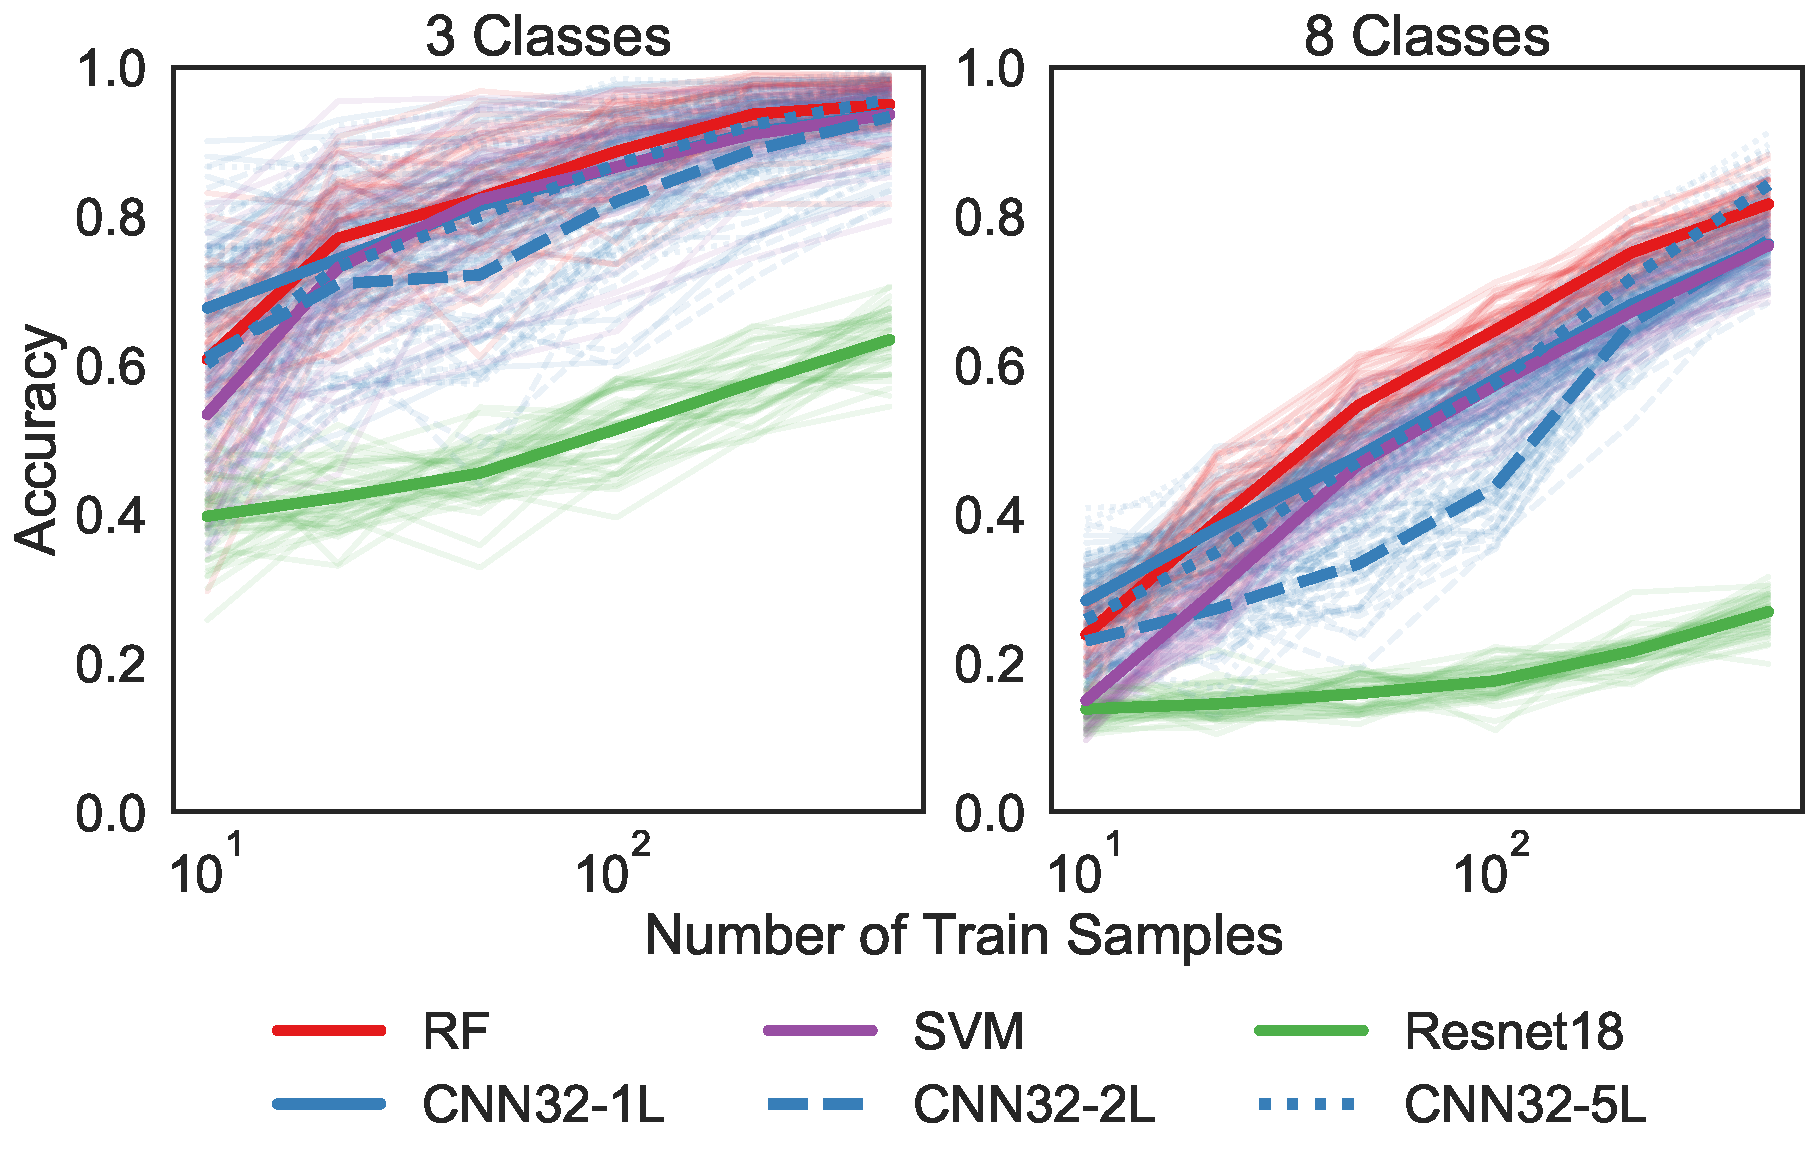
\includegraphics[width=0.6\textwidth]{figures/mel.pdf}
  \caption{Performance of RF, SVM-RBF, and DN on multiclass FSDD classifications using mel-spectrogram.
  The y-axes represent classifier accuracy on a linear scale and the x-axes correspond to logarithmic sample sizes from 10 to 480. Each panel shows average results over 45 random class combinations and individual trajectories with lower alpha
  In the 3-class task, RF, SVM, 1-layer, and 5-layer CNNs all have very similar performances. In the 8-class task, RF achieves the highest accuracy. ResNet-18-Audio performs much worse than other classifiers.
  }
\label{fig:mel}
\end{figure}
\vfil\eject

\section{FSDD Benchmarks with MFCC}
\label{mfcc}
As an alternative conversion, we used PyTorch’s inbuilt function and converted the raw audio magnitudes into MFCC \citep{pytorch}. The process calculated MFCC on the DB-scaled mel-spectrograms. The results (Figure \ref{fig:mfcc}) were qualitatively similar to FSDD benchmarks with spectrogram (Figure \ref{fig:spoken_digit}) and mel-spectrogram (Figure \ref{fig:mel}) conversions.

\begin{figure}[!htb]
\centering
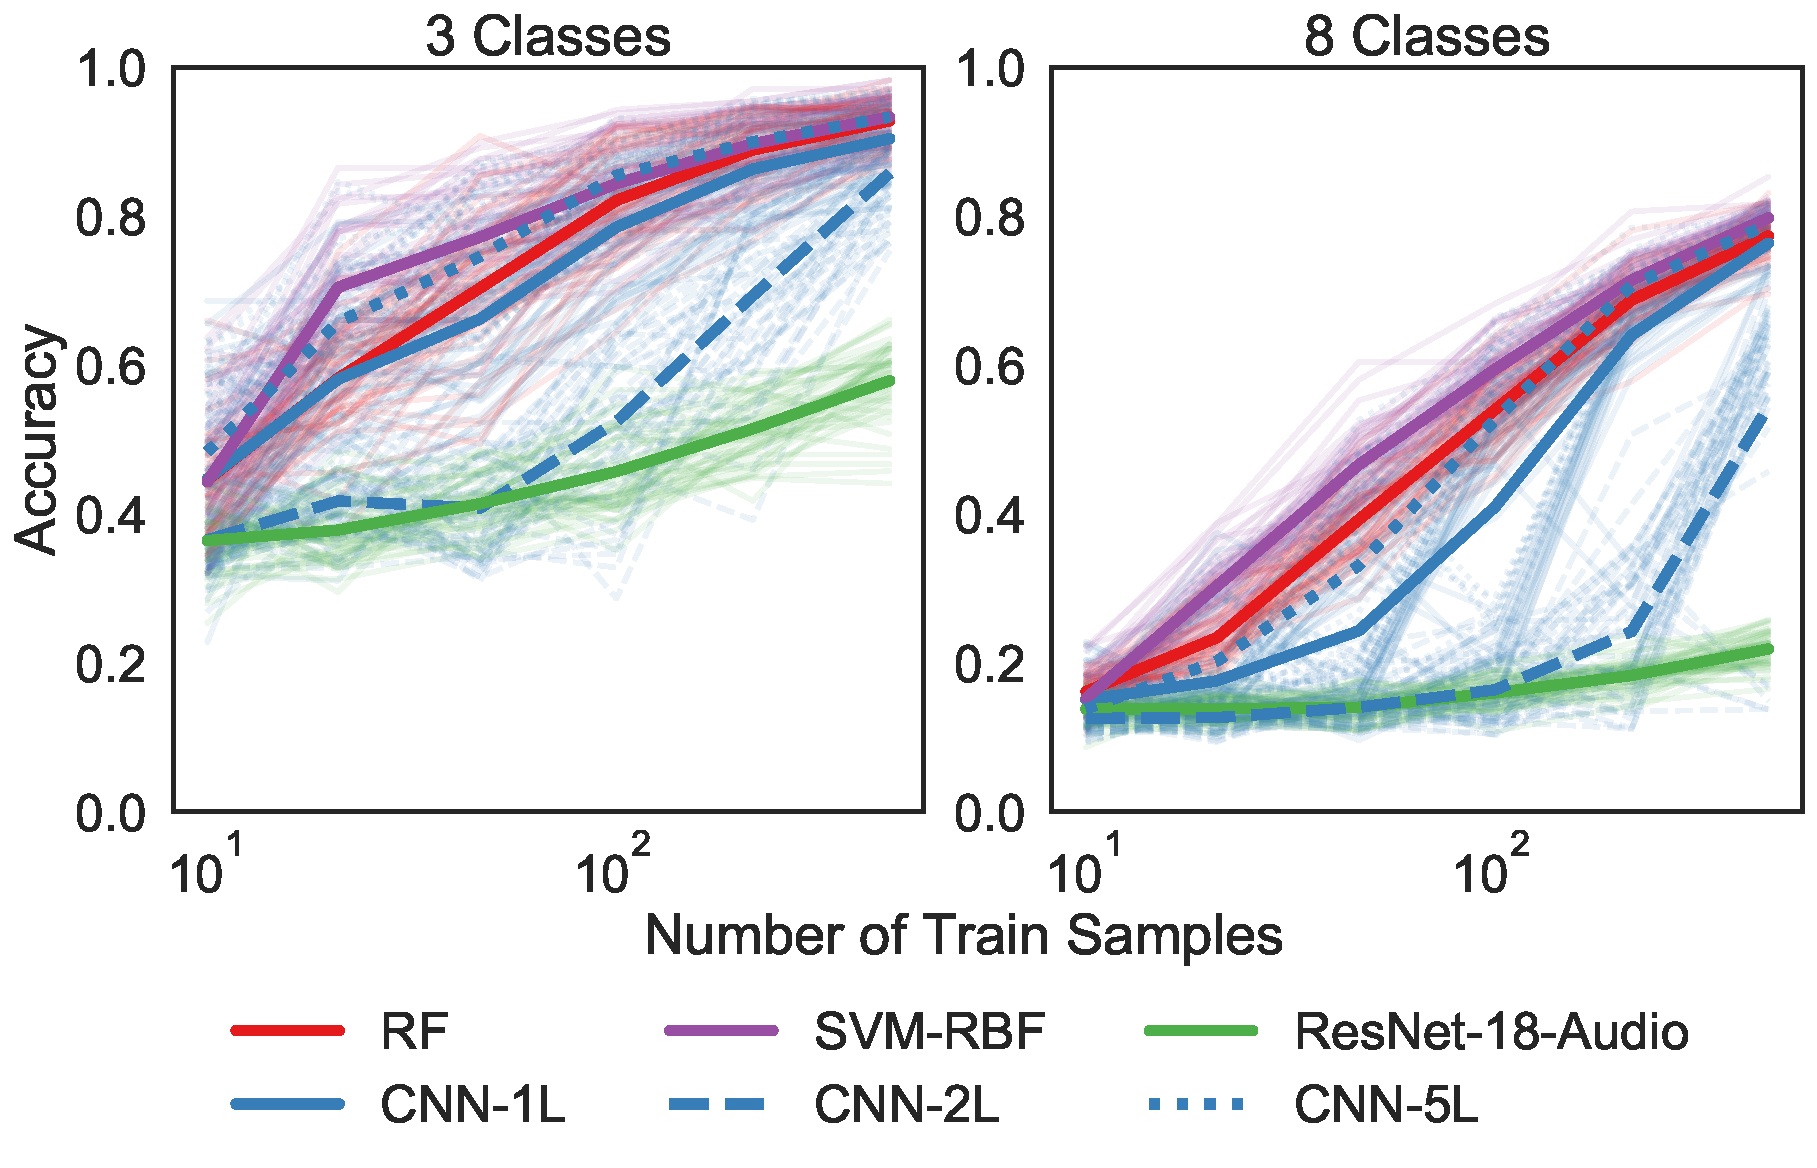
\includegraphics[width=0.6\textwidth]{figures/mfcc.pdf}
  \caption{Performance of RF, SVM-RBF, and DN on multiclass FSDD classifications using mel-frequency cepstral coefficients (MFCC). 
  The y-axes represent classifier accuracy on a linear scale and the x-axes correspond to logarithmic sample sizes from 10 to 480. Each panel shows average results over 45 random class combinations and individual trajectories with lower alpha.
  SVM-RBF achieved the best performance in both tasks, but the advantage diminishes as the sample size increases. At the maximum sample size, RF, SVM, 1-layer, and 5-layer CNNs all have very similar accuracy. 2-layer CNN performs worse, while ResNet-18-Audio performs the worst.
  }
\label{fig:mfcc}
\end{figure}
\vfil\eject